\section{Artefact}\label{sec:artefact}
This section describes the NetLogo model created, `FoodDelivery'.

The world being modeled is what is known as the last mile in the food delivery industry.
This term is used for the last step in the delivery of online-ordered goods.

Companies in the food delivery industry offer services to three parties:
\begin{enumerate}
    \item Restaurants sell their food in a portal created by the delivery company.
    \item Consumers buy food from a restaurant using the same portal.
    \item Deliverers use an app that assigns deliveries and gives route directions.
\end{enumerate}

Some key steps in the food ordering and delivery process, and of interest for this study, are:
\begin{itemize}
    \item A hungry customer orders a meal in the portal at a restaurant.
    \item The restaurant starts preparing the meal; this may take some time (say, on average, 10 minutes).
    \item When it starts preparing, a deliverer is needed, announced in the deliverers' app.
    \item A deliverer can claim the delivery (or is assigned) and starts cycling towards the restaurant.
    \item When the deliverer arrives at the restaurant, it may have to wait until the meal is ready.
    \item When the meal is ready, the deliverer accepts it and starts driving towards the customer.
    \item It is possible no deliverer is available, or it takes too long to get to the restaurant,
then the meal will be thrown away.
    \item If the meal gets delivered, the customer is happy
    \item If the meal is not delivered, the customer and the restaurant are unhappy.
    \item If a customer is unhappy, it will eventually stop ordering meals.
    \item If a restaurant is unhappy, it will eventually stop using the service.
\end{itemize}

This all takes place in a city with restaurants and customers.
The deliverers have to cycle to the restaurant and then to the customer.
The best route will be provided by the app a deliverer uses.

The money for the delivery company is earned by charging the restaurants per delivery.
The company's interest is thus to have as many deliveries as possible; this means they want happy customers and enough deliverers to keep them happy.

The above process is more or less how the process works in the real world.

\subsection{Conceptional model}\label{subsec:conceptional-model}
The FoodDelivery model has the same types of agents:
\begin{enumerate}
\item deliverers
\item restaurants
\item customers
\end{enumerate}

The delivery company itself is not modeled explicitly; they are what is called the observer.

\paragraph{Customers}
In a city, locals can order food using the deliverer's site.

Orders are not equally distributed over the day: peak hours are breakfast, lunch, and mostly dinner.
The order probability distribution from the model is shown in figure~\ref{fig:food_ordering_distribution}.

\begin{figure}
    \centering
    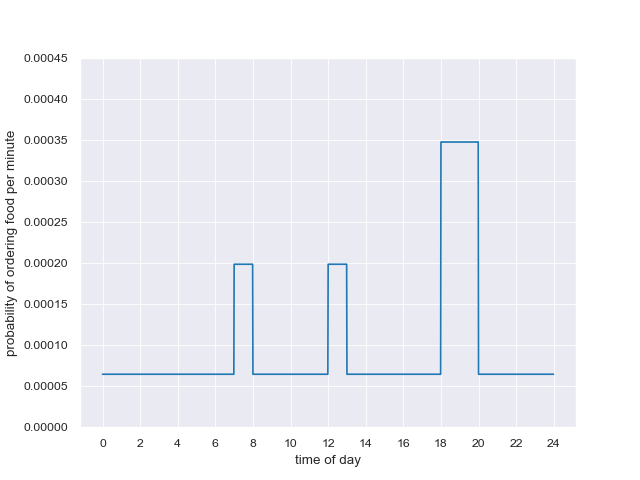
\includegraphics[width=8.5cm]{sections/pics/food_ordering_distribution}
    \caption{food ordering probabilities for one day}
    \label{fig:food_ordering_distribution}
\end{figure}

When a customer orders a meal but it does not get delivered, he or she is disappointed, and if that happens again, the customer will stop using the delivery site.
The possible restaurants must fall within a certain radius of the customer.

In the model, the number of possible customers can be set.
They are randomly distributed over the map.
When no restaurant falls in an adjustable radius from the customer, the customer is removed.

The restaurant is randomly selected in a given radius when ordering a meal.
When no restaurant is within the given radius, the customer will disappear.

If a meal is not delivered, the customer is unsatisfied, and their satisfaction level is subtracted 1 point.
Customers stop ordering food if they have a satisfaction level below -1.

In short:
\begin{itemize}
\item number of possible customers can be set, customers are randomly distributed over the map
\item customers order on average once a week following the probability distribution shown in figure~\ref{fig:food_ordering_distribution}
\item customers with no restaurants nearby (radius can be set) will stop ordering (disappear from the world)
\item customers who don't receive their ordered meal are unhappier (happiness -1)
\item customers who receive their ordered meal are happier (happiness +1)
\item unhappy customers stop ordering (disappear from the world)
\item max happiness = 1
\item min happiness = -1
\item stop if happiness \textless -1
\end{itemize}

\paragraph{Restaurants}
In a city, restaurants exist that may use the delivery companies' services.

In the model, the number of restaurants can be set.
They are randomly distributed over the map.

When an order arrives, the preparation starts.
The preparation time is Gaussian distributed, and the mean and standard deviation can be set.
To simulate the different preparation times.

Upon order arrival, the meal can be assigned to a deliverer.
The assignment in the real world is done with an algorithm that combines several factors.

In the model, the simplified possibilities are:
\begin{enumerate}
\item equally distribute the orders among the deliverers
\item or assign it to the closest free deliverer
\end{enumerate}

When the meal is ready, it can be picked up within a waiting time, which is a variable that can be set.
After this waiting time, the meal will be thrown away.
Throwing away a meal costs the restaurant money. If this happens, the restaurant will become unhappy and may stop using the service.

In short:
\begin{itemize}
\item the number of restaurants can be set; they are randomly distributed on the map
\item meals have a normal distributed preparation time that can be set
\item meals have a pickup time, within the meal must be picked up
\item after the pickup time, the meal is discarded
\item a discarded meal makes the restaurant unhappy
\item if in a week more meals are discarded than delivered, the restaurant stops using the service
\end{itemize}

\paragraph{Deliverers}
Deliverers are people who choose to work for a deliverer company.
Some companies provide them with the equipment (usually when the drivers are hired as employees), while others
let them use (and even buy) their required equipment.

The hiring part is not in the model.
At the start of the simulation, the number of deliverers is set.
The number of deliverers can only decline.

When a meal is assigned to the deliverer, it will take the shortest route
to the restaurant, waits until the meal is ready, and moves to the customer.

The deliverer will lose its assigned meal if they do not arrive before the waiting time is over.
A deliverer can only receive or deliver a meal when it is neighboring a restaurant or the customer.

As a design choice, deliverers have no shifts; they always work.
Using shifts would make the model much more complicated; this could be done in the next version.

In short:

\begin{itemize}
\item the number of deliverers can be set; they are randomly distributed over the map
\item assignment of meals:
\begin{itemize}
      \item a free deliverer is assigned fair (every deliverer gets the same number of jobs)
      \item or a free deliverer is assigned to the closest unassigned meal.
\end{itemize}
\item employment method:
\begin{itemize}
      \item the number of deliverers is stable when they are hired as employees
      \item or number of delivers may decline if they deliver not enough in a week,
    if they do not make enough deliveries in a week, they have a 50\% chance of leaving
\end{itemize}
\end{itemize}

\paragraph{The world}
Most delivery companies operate in densely populated areas.
In that area, blocks exist for buildings, in our case the restaurants and customer buildings.
And the buildings are connected with roads.
The roads are divided in a left side and a right side, and crossings exist.

The model consists of a grid of squares; some squares will be blocks of buildings, and others represent the streets.
This grid places restaurants and customers randomly on the building blocks.
The deliverers are initially randomly placed on the streets; they can only move on the street patches.

\subsection{Computer model}\label{subsec:computer-model}
The world is, for a large part, built using the code from the Taxi Cab model.
The streets and how the deliveries move are from their model; only the traffic lights were removed.

The design of the grid is shown in figure~\ref{fig:grid}.
\begin{center}
\begin{figure*}
    \centering
    \begin{subfigure}[m]{0.8\textwidth}
        \centering
        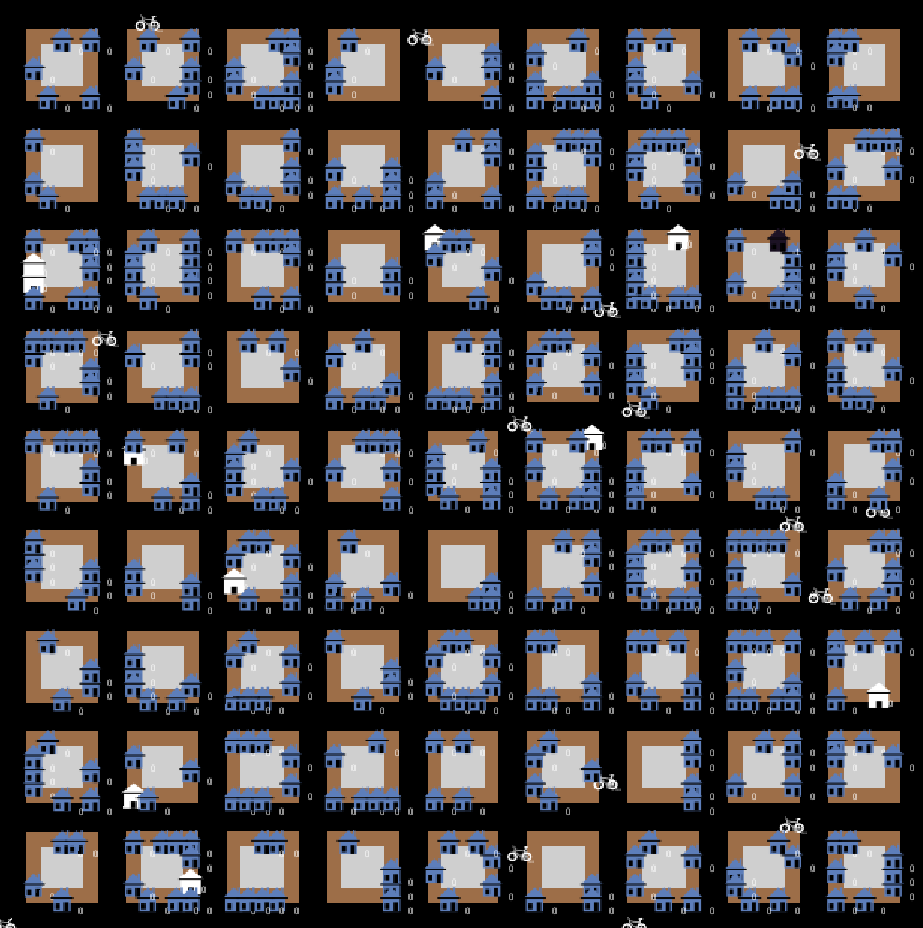
\includegraphics[width=8cm]{sections/pics/grid}
        \caption{FoodDelivery grid}
    \end{subfigure}
    \hfill
    \begin{subfigure}[m]{0.8\textwidth}
        \centering
        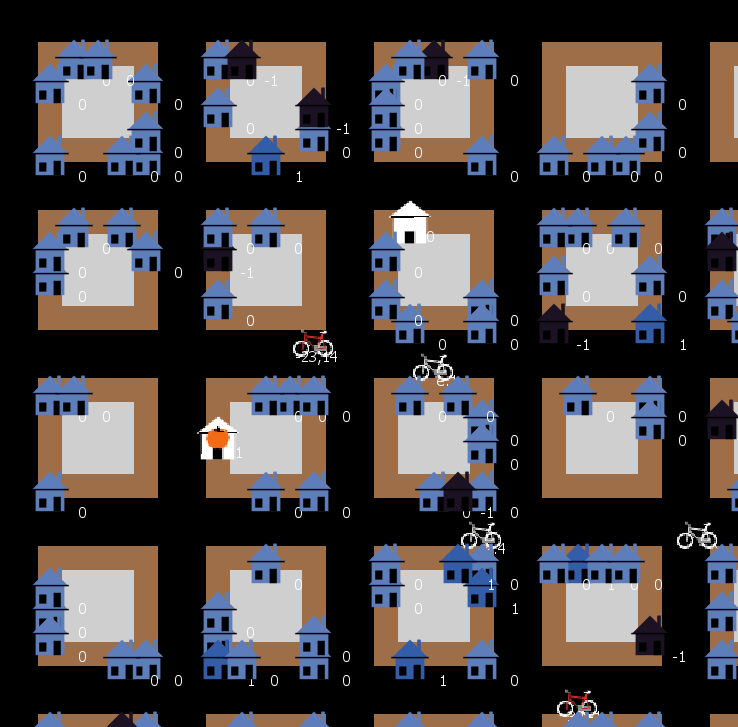
\includegraphics[width=8cm]{sections/pics/grid_closeup}
        \caption{Fooddelivery grid closeup}
    \end{subfigure}
    \caption{FoodDelivery grid}
    \label{fig:grid}
\end{figure*}

\end{center}
The agent's design is shown in figure~\ref{fig:agents}.
\begin{center}
\begin{figure}
     \centering
     \begin{subfigure}[m]{0.1\textwidth}
         \centering
         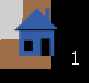
\includegraphics[width=\textwidth]{sections/pics/cust_happy}
         \caption{Customer with happiness score}
     \end{subfigure}
     \hfill
     \begin{subfigure}[m]{0.1\textwidth}
         \centering
         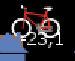
\includegraphics[width=\textwidth]{sections/pics/del_on_its_way}
         \caption{Deliverer on route to loc 23,1}
     \end{subfigure}
     \hfill
     \begin{subfigure}[m]{0.1\textwidth}
         \centering
         
\includegraphics[width=\textwidth]{sections/pics/meal_prep}
         \caption{Restaurant with a meal ordered on top and number of ordered}
     \end{subfigure}
      \hfill
     \begin{subfigure}[m]{0.1\textwidth}
         \centering
         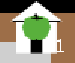
\includegraphics[width=\textwidth]{sections/pics/meal_ready}
         \caption{Restaurant with a meal ready on top and number of ordered}
     \end{subfigure}
        \caption{Agents examples}
        \label{fig:agents}
\end{figure}
\end{center}
In NetLogo, everything works on ticks; all code in the go procedure is executed during one tick.
The programmer must decide what to do and not to do in that tick during programming.
And be sure that each agent does only one thing in a tick.

In one tick, all behavior of one kind of agent is executed in series.
The order of these series is essential.

This system makes it difficult to program future behavior as each agent decides only its behavior one tick at a time.
For example, moving towards a restaurant means moving to an allowed patch that minimizes the distance to that restaurant.

The most important parts of the grid are the squares.
The squares are named patches.

The street patches have four kinds:\\
- right patches where a deliverer can only move right\\
- left patches where a deliverer can only move left\\
- up patches where a deliverer can only move up\\
- down patches where a deliverer can only move down\\

On horizontal roads, the allowed directions are left or right
On vertical roads, the directions are up or down.

Next to road patches, there are intersection patches; on these patches, a driver has more allowed directions.
These are:\\
- up or right\\
- up or left\\
- left or down\\
- right or down\\

At an intersection, a deliverer decides which direction to go.
To get to the other side of the road, the deliverer must make a U-turn at an intersection.

Special patches are the intersections at the grid's edges; a deliverer can not leave the grid.

Another important detail is that to pick up or deliver a meal; the delivery person must be on a street patch rather than at an intersection.

The program is available inside a git repository available at GitHub~\footnote{\url{https://github.com/evertvankammen/FooddeliveryNetlogo}}
This repository also contains the Python code to automate the model's running with different parameters.h and not on an intersection.